\documentclass[a4paper, UKenglish, 11pt]{uiomaster}
\usepackage{lipsum}
\usepackage[subpreambles=true]{standalone}

\begin{document}

\chapter{Dipole Source Localization using Neural Networks}
In this chapther we will be presenting the neural networks used for the localization of current dipole sources in the human cortex.


\subsubsection{Feed Forward Neural Networks}
The feedforward neural network (FFNN) was one of the first artificial neural network to be adopted and is yet today an important algorithm used in machine learning. The feed forward neural network is the simplest form of neural network, as information is only processed forward, from the input nodes, through the hidden nodes and to the output nodes \cite{Hjorth-Jensen2022}.


\subsubsection{Convolutional Neural Networks}
Convolutional neural networks (CNNs) is an other variant of FFNNs that have drawen inspiration from the functioning of the visual cortex of the brain. In the visual cortex, individual neurons exhibit selective responses to stimuli within small sub-regions of the visual field, known as receptive fields. This property allows the neurons to effectively exploit the spatially local correlations present in natural images. Mathematically, the response of each neuron can be approximated using a convolution operation \cite{Hjorth-Jensen2022}.

% TODO: check sources
CNNs mimic the behavior of visual cortex neurons by utializing a specific connectivity pattern between nodes in adjacent layers. Unlike fully contected FFNNs, where each node connects to all nodes in the preceding layer, CNNs  local connectivity. In other words, each node in a convolutional layer is only connected to a subset of nodes in the previous layer. Typically, CNNs consist of multiple convolutional layers that learn local features from the input data. These layers are followed by a fully connected layer that combines the learned local information to produce the final outputs. CNNs find wide applications in image and video recognition tasks \cite{Hjorth-Jensen2022}.

\subsection{Neural Networks}
Artificial Neural Networks are computational systems that can learn to perform tasks by considering examples, generally without being programmed with any task-specific rules \cite{101}.

The biological neural networks of animal brains, wherein neurons interact by sending signals in the form of mathematical functions between layers, has inspired a simple model for an artificial neuron:

\begin{equation}
    a = f \left( \Sigma_{i=1}^n w_ix_i + b_i\right ) = f(z)
    \label{eq:NN}
\end{equation}

where the output $a$ of the neuron is the value of its activation function $f$, which as input has the sum of signals $x_i, x_{i+1}, ..., x_n$ received by $n$ other neurons, multiplied with the weights $w_i, w_{i+1}, ..., w_n$ and added with biases.

Most artificial neural networks consists of an input layer, an output layer and layers in between, called hidden layers. The layers consists of an arbitrary number of neurons, also referred to as nodes. The connection between two nodes is associated with a weight variable $w$, that weights the importance of various inputs. A more convenient notation for the activation function is:

\begin{equation}
    a_i(\boldsymbol{x}) = f_i(z^{(i)}) = f_i(\boldsymbol{w^{i}}\cdot \boldsymbol{x} + b^{i})
\label{eq:NN_vec}
\end{equation}

where $\boldsymbol{w}^{(i)} = (w_1^{(i)}, w_2^{(i)}, ..., w_n^{(i)})$ and $b^{(i)}$ are the neuron-specific weights and biases respectively. The bias is normally needed in case of zero activation weights or inputs \cite{101}.

\section{Feed-Forward Neural Network Approach for localizing single dipole sources}
The feedforward neural network (FFNN) was one of the first artificial neural network to be adopted and is yet today an important algorithm used in machine learning. The feed forward neural network is the simplest form of neural network, as information is only processed forward, from the input nodes, through the hidden nodes and to the output nodes.



\subsection{DiLoc}
The FFNN that are trained to solve the inverse problem of ours has an input layer of 231 neurons, corresponding to the M = 231 electrode measures of the potentials. The input layer is followed by three hidden layers with 120, 84 and 16 hidden neurons, respectively. When the aim is to estimate the localization of the current dipole, \emph{only}, the final output layer holds the predicted x-, y- and z- position of the desired dipole source.  However, if the interest lies in determining the size of the dipole population, an alternative output layer is incorporated in the network architecture providing the radius of the dipole(s), in addition to the location coordinates. This enables the model to provide a more comprehensive understanding of the dipole source(s) being analyzed.

\begin{figure}
  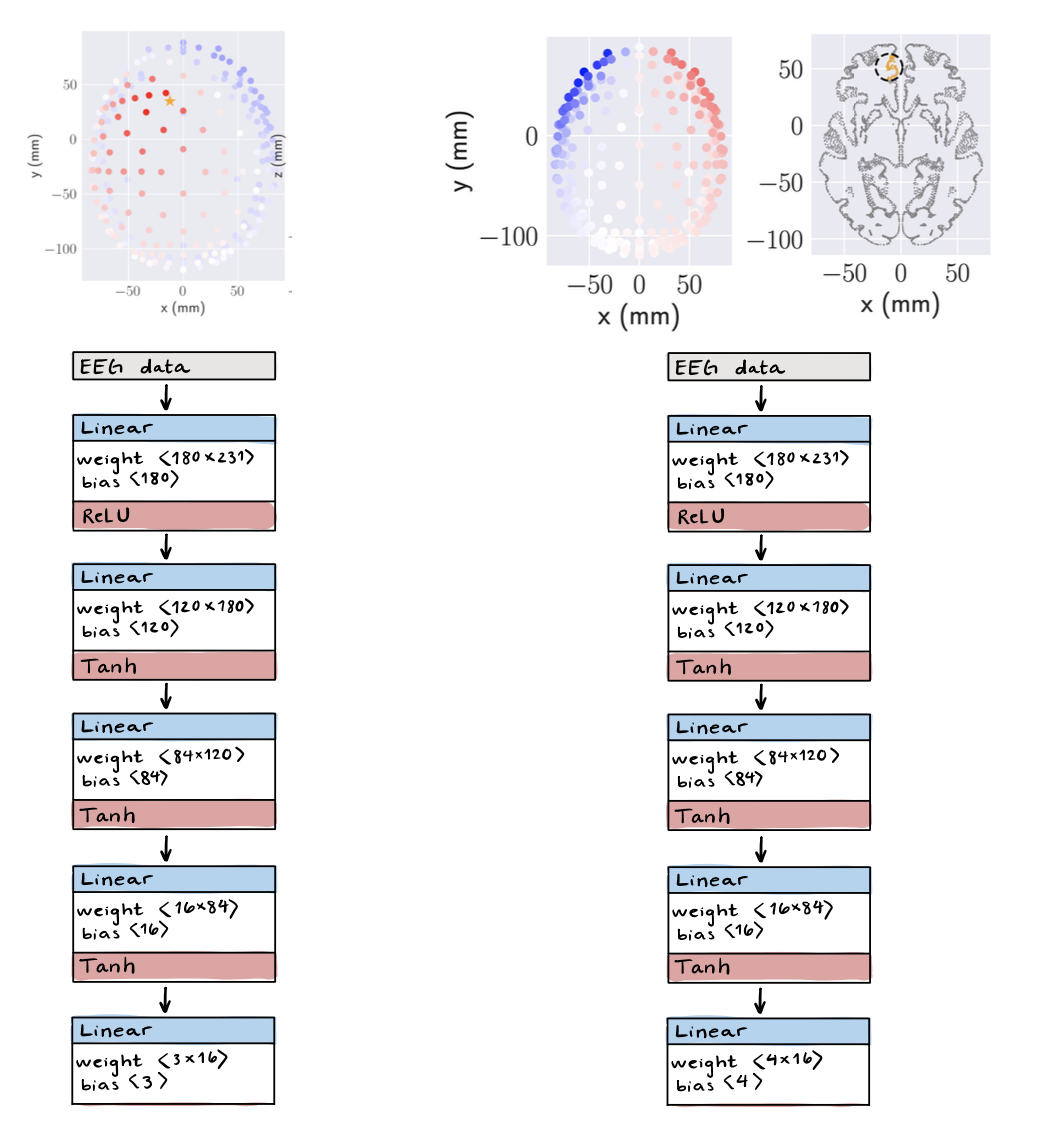
\includegraphics[width=\linewidth]{figures/NN_architecture.png}
  \caption{A caption here is needed.}
  \label{fig:NN_architecture.png}
\end{figure}

\subsection{Validation accuracy}
In Figure \ref{fig:single_dipole_accuracy} we have provided the validation accuray, using mean squared error (MSE) and the coefficient of determination (R2-score).

The expression for MSE when predicting the x-, y- and z-coordinate, goes as follows:

\begin{equation}
MSE(\hat{y},\hat{\tilde{y}}) = \frac{1}{n}
\sum_{i=1}^{n}(y_i-\tilde{y}_i)^2 \\
= \frac{1}{3}\sum_{i=1}^{3}((x-\tilde{x})^2 + (y-\tilde{y})^2 + (z-\tilde{z})^2 )
\label{eq:MSE}
\end{equation}

The coefficient of determination is given as follows:
\begin{equation}
R^2(\hat{y}, \tilde{\hat{y}}) = 1 - \frac{\sum_{i=0}^{n - 1} (y_i - \tilde{y}_i)^2}{\sum_{i=0}^{n - 1} (y_i - \bar{y})^2},
\label{eq:R2}
\end{equation}

Where the mean value of $y_i$ is defined by $\bar{y}$:

\begin{equation*}
\bar{y} =  \frac{1}{n} \sum_{i=0}^{n - 1} y_i.
\label{eq:ybar}
\end{equation*}



\subsection{Activation functions, Batchsize and Optimization}
For the neurons of the input layers we use the linear activation function ReLu, while for the neurons of the hidden and output layers, we chose the much used hyperbolic tangent activation function.

Cost function
% Maybe this does not belong here?
In order to train the network faster, one commonly split the data set into mini-batches, which is also done here. When splitting the data such a way, the weights of connection between neurons are updated after each propagation, making the network converge considerable faster.

Scaling
Every potential distribution presented to the network is first average referenced by subtracting the average of all potential values. Subsequently, the average referenced potentials are normalized by dividing them by the magnitude of the largest. The dipole location parameters are normalized to 1 with respect to the radius of the outer head boundary in the spherical head model (9.2 cm). In the case of a realistically shaped head model, the location parameters are normalized with respect to the radius of the best-fitting sphere for the scalp–air interface.

As was pointed out in the previous section, the optimal dipole orientation (in the leastsquares sense) for a given location can be calculated in a straightforward manner. Therefore, we will use neural networks to estimate only the dipole location parameters.


\subsection{Training, testing and evaluation}
In order to make an ANN that generalizes well to new data we split our data into training and testing sets. Randomly selecting 80 percent of the rows in the full dataset, we put this into a separate one and call it our training set. The remaining 20 percent is put into the test set. In practice, the training data set consists of pairs of an input vector with EEG signals and the corresponding output vector, where the answer key is the x-, y- and z coordinate of the dipole source. The neural network is then feed with the training data and produces an estimation of the localization of the dipole. The estimation is found by the network through optimizing the parameters $\beta$ minimizing the cost function, or said in other words, through finding parameters for the function that produces the smallest outcomes, meaning the smallest errors. The result provided by the network is then compared with the target, for each input vector in the training data. Adjustment of parameters...

When the network is fully trained, we have a final model fit on the training data set. Feeding the network with the test data set, we can assess the performance of the network. The predictions of the fully trained network can now be compared to the holdout data's true values to determine the model's accuracy.

In figure \ref{fig:single_dipole_accuracy_FFNN} we have provided the bias-variance trade-off for when using Tanh as activation function. We notice that error of the model is approaching 0 and that the variance between the two curves decreases for an increasing number of epochs.


% Notes:
% The ‘lead field’ or ‘forward model’ used for EEG inverse
% modeling relates a current source in the brain to the electric potentials
% measured on the scalp (Sarvas, 1987; Mosher et al., 1999; Baillet et al.,
% 2001; Vatta et al., 2010; Akalin Acar and Makeig, 2013; Vorwerk et al.,
% 2014).


\end{document}